\documentclass[a4paper,10pt]{article} % Uses article class in A4 format

%%%%%%%%%%%%%%%%%%%%%%%%%%%%%%%%%%%%%%%%%
% The Legrand Orange Book
% Structural Definitions File
% Version 2.0 (9/2/15)
%
% Original author:
% Mathias Legrand (legrand.mathias@gmail.com) with modifications by:
% Vel (vel@latextemplates.com)
% 
% This file has been downloaded from:
% http://www.LaTeXTemplates.com
%
% License:
% CC BY-NC-SA 3.0 (http://creativecommons.org/licenses/by-nc-sa/3.0/)
%
%%%%%%%%%%%%%%%%%%%%%%%%%%%%%%%%%%%%%%%%%

%----------------------------------------------------------------------------------------
%	VARIOUS REQUIRED PACKAGES AND CONFIGURATIONS
%----------------------------------------------------------------------------------------

\usepackage[top=3cm,bottom=3cm,left=3cm,right=3cm,headsep=10pt,a4paper]{geometry} % Page margins

\usepackage{caption}
\usepackage{mathtools}
\usepackage{subfigure}
\usepackage{cancel}
\usepackage{colortbl}
\usepackage{steinmetz}
\usepackage{diffcoeff}

\usepackage{graphicx} % Required for including pictures
\graphicspath{{Pictures/}} % Specifies the directory where pictures are stored

\usepackage{lipsum} % Inserts dummy text

\usepackage{tikz} % Required for drawing custom shapes

\usepackage[spanish]{babel} % English language/hyphenation

\usepackage{enumitem} % Customize lists
\setlist{nolistsep} % Reduce spacing between bullet points and numbered lists

\usepackage{booktabs} % Required for nicer horizontal rules in tables

\usepackage{xcolor} % Required for specifying colors by name
\definecolor{ocre}{RGB}{52,177,201} % Define the orange color used for highlighting throughout the book

%----------------------------------------------------------------------------------------
%	FONTS
%----------------------------------------------------------------------------------------

\usepackage{avant} % Use the Avantgarde font for headings
%\usepackage{times} % Use the Times font for headings
\usepackage{mathptmx} % Use the Adobe Times Roman as the default text font together with math symbols from the Sym­bol, Chancery and Com­puter Modern fonts

\usepackage{microtype} % Slightly tweak font spacing for aesthetics
\usepackage[utf8]{inputenc} % Required for including letters with accents
\usepackage[T1]{fontenc} % Use 8-bit encoding that has 256 glyphs

%----------------------------------------------------------------------------------------
%	BIBLIOGRAPHY AND INDEX
%----------------------------------------------------------------------------------------

\usepackage[style=alphabetic,citestyle=numeric,sorting=nyt,sortcites=true,autopunct=true,babel=hyphen,hyperref=true,abbreviate=false,backref=true,backend=biber]{biblatex}
\addbibresource{bibliography.bib} % BibTeX bibliography file
\defbibheading{bibempty}{}

\usepackage{calc} % For simpler calculation - used for spacing the index letter headings correctly
\usepackage{makeidx} % Required to make an index
\makeindex % Tells LaTeX to create the files required for indexing

%----------------------------------------------------------------------------------------
%	MAIN TABLE OF CONTENTS
%----------------------------------------------------------------------------------------

\usepackage{titletoc} % Required for manipulating the table of contents

\contentsmargin{0cm} % Removes the default margin

% Part text styling
\titlecontents{part}[0cm]
{\addvspace{20pt}\centering\large\bfseries}
{}
{}
{}

% Chapter text styling
\titlecontents{chapter}[1.25cm] % Indentation
{\addvspace{12pt}\large\sffamily\bfseries} % Spacing and font options for chapters
{\color{ocre!60}\contentslabel[\Large\thecontentslabel]{1.25cm}\color{ocre}} % Chapter number
{\color{ocre}}  
{\color{ocre!60}\normalsize\;\titlerule*[.5pc]{.}\;\thecontentspage} % Page number

% Section text styling
\titlecontents{section}[1.25cm] % Indentation
{\addvspace{3pt}\sffamily\bfseries} % Spacing and font options for sections
{\contentslabel[\thecontentslabel]{1.25cm}} % Section number
{}
{\hfill\color{black}\thecontentspage} % Page number
[]

% Subsection text styling
\titlecontents{subsection}[1.25cm] % Indentation
{\addvspace{1pt}\sffamily\small} % Spacing and font options for subsections
{\contentslabel[\thecontentslabel]{1.25cm}} % Subsection number
{}
{\ \titlerule*[.5pc]{.}\;\thecontentspage} % Page number
[]

% List of figures
\titlecontents{figure}[0em]
{\addvspace{-5pt}\sffamily}
{\thecontentslabel\hspace*{1em}}
{}
{\ \titlerule*[.5pc]{.}\;\thecontentspage}
[]

% List of tables
\titlecontents{table}[0em]
{\addvspace{-5pt}\sffamily}
{\thecontentslabel\hspace*{1em}}
{}
{\ \titlerule*[.5pc]{.}\;\thecontentspage}
[]

%----------------------------------------------------------------------------------------
%	MINI TABLE OF CONTENTS IN PART HEADS
%----------------------------------------------------------------------------------------

% Chapter text styling
\titlecontents{lchapter}[0em] % Indenting
{\addvspace{15pt}\large\sffamily\bfseries} % Spacing and font options for chapters
{\color{ocre}\contentslabel[\Large\thecontentslabel]{1.25cm}\color{ocre}} % Chapter number
{}  
{\color{ocre}\normalsize\sffamily\bfseries\;\titlerule*[.5pc]{.}\;\thecontentspage} % Page number

% Section text styling
\titlecontents{lsection}[0em] % Indenting
{\sffamily\small} % Spacing and font options for sections
{\contentslabel[\thecontentslabel]{1.25cm}} % Section number
{}
{}

% Subsection text styling
\titlecontents{lsubsection}[.5em] % Indentation
{\normalfont\footnotesize\sffamily} % Font settings
{}
{}
{}

%----------------------------------------------------------------------------------------
%	PAGE HEADERS
%----------------------------------------------------------------------------------------

\usepackage{fancyhdr} % Required for header and footer configuration

\pagestyle{fancy}
\renewcommand{\chaptermark}[1]{\markboth{\sffamily\normalsize\bfseries\chaptername\ \thechapter.\ #1}{}} % Chapter text font settings
\renewcommand{\sectionmark}[1]{\markright{\sffamily\normalsize\thesection\hspace{5pt}#1}{}} % Section text font settings
\fancyhf{} \fancyhead[LE,RO]{\sffamily\normalsize\thepage} % Font setting for the page number in the header
\fancyhead[LO]{\rightmark} % Print the nearest section name on the left side of odd pages
\fancyhead[RE]{\leftmark} % Print the current chapter name on the right side of even pages
\renewcommand{\headrulewidth}{0.5pt} % Width of the rule under the header
\addtolength{\headheight}{2.5pt} % Increase the spacing around the header slightly
\renewcommand{\footrulewidth}{0pt} % Removes the rule in the footer
\fancypagestyle{plain}{\fancyhead{}\renewcommand{\headrulewidth}{0pt}} % Style for when a plain pagestyle is specified

% Removes the header from odd empty pages at the end of chapters
\makeatletter
\renewcommand{\cleardoublepage}{
\clearpage\ifodd\c@page\else
\hbox{}
\vspace*{\fill}
\thispagestyle{empty}
\newpage
\fi}

%----------------------------------------------------------------------------------------
%	THEOREM STYLES
%----------------------------------------------------------------------------------------

\usepackage{amsmath,amsfonts,amssymb,amsthm} % For math equations, theorems, symbols, etc

\newcommand{\intoo}[2]{\mathopen{]}#1\,;#2\mathclose{[}}
\newcommand{\ud}{\mathop{\mathrm{{}d}}\mathopen{}}
\newcommand{\intff}[2]{\mathopen{[}#1\,;#2\mathclose{]}}
\newtheorem{notation}{Notation}[chapter]

% Boxed/framed environments
\newtheoremstyle{ocrenumbox}% % Theorem style name
{0pt}% Space above
{0pt}% Space below
{\normalfont}% % Body font
{}% Indent amount
{\small\bf\sffamily\color{ocre}}% % Theorem head font
{\;}% Punctuation after theorem head
{0.25em}% Space after theorem head
{\small\sffamily\color{ocre}\thmname{#1}\nobreakspace\thmnumber{\@ifnotempty{#1}{}\@upn{#2}}% Theorem text (e.g. Theorem 2.1)
\thmnote{\nobreakspace\the\thm@notefont\sffamily\bfseries\color{black}---\nobreakspace#3.}} % Optional theorem note
\renewcommand{\qedsymbol}{$\blacksquare$}% Optional qed square

\newtheoremstyle{blacknumex}% Theorem style name
{5pt}% Space above
{5pt}% Space below
{\normalfont}% Body font
{} % Indent amount
{\small\bf\sffamily}% Theorem head font
{\;}% Punctuation after theorem head
{0.25em}% Space after theorem head
{\small\sffamily{\tiny\ensuremath{\blacksquare}}\nobreakspace\thmname{#1}\nobreakspace\thmnumber{\@ifnotempty{#1}{}\@upn{#2}}% Theorem text (e.g. Theorem 2.1)
\thmnote{\nobreakspace\the\thm@notefont\sffamily\bfseries---\nobreakspace#3.}}% Optional theorem note

\newtheoremstyle{blacknumbox} % Theorem style name
{0pt}% Space above
{0pt}% Space below
{\normalfont}% Body font
{}% Indent amount
{\small\bf\sffamily}% Theorem head font
{\;}% Punctuation after theorem head
{0.25em}% Space after theorem head
{\small\sffamily\thmname{#1}\nobreakspace\thmnumber{\@ifnotempty{#1}{}\@upn{#2}}% Theorem text (e.g. Theorem 2.1)
\thmnote{\nobreakspace\the\thm@notefont\sffamily\bfseries---\nobreakspace#3.}}% Optional theorem note

% Non-boxed/non-framed environments
\newtheoremstyle{ocrenum}% % Theorem style name
{5pt}% Space above
{5pt}% Space below
{\normalfont}% % Body font
{}% Indent amount
{\small\bf\sffamily\color{ocre}}% % Theorem head font
{\;}% Punctuation after theorem head
{0.25em}% Space after theorem head
{\small\sffamily\color{ocre}\thmname{#1}\nobreakspace\thmnumber{\@ifnotempty{#1}{}\@upn{#2}}% Theorem text (e.g. Theorem 2.1)
\thmnote{\nobreakspace\the\thm@notefont\sffamily\bfseries\color{black}---\nobreakspace#3.}} % Optional theorem note
\renewcommand{\qedsymbol}{$\blacksquare$}% Optional qed square
\makeatother

% Defines the theorem text style for each type of theorem to one of the three styles above
\newcounter{dummy} 
\numberwithin{dummy}{section}
\theoremstyle{ocrenumbox}
\newtheorem{theoremeT}[dummy]{Theorem}
\newtheorem{problem}{Problem}[chapter]
\newtheorem{exerciseT}{Ejemplo}[chapter]
\theoremstyle{blacknumex}
\newtheorem{exampleT}{Ejemplo}[chapter]
\theoremstyle{blacknumbox}
\newtheorem{vocabulary}{Vocabulary}[chapter]
\newtheorem{definitionT}{Definition}[section]
\newtheorem{corollaryT}[dummy]{Corollary}
\theoremstyle{ocrenum}
\newtheorem{proposition}[dummy]{Proposition}

%----------------------------------------------------------------------------------------
%	DEFINITION OF COLORED BOXES
%----------------------------------------------------------------------------------------

\RequirePackage[framemethod=default]{mdframed} % Required for creating the theorem, definition, exercise and corollary boxes

% Theorem box
\newmdenv[skipabove=7pt,
skipbelow=7pt,
backgroundcolor=black!5,
linecolor=ocre,
innerleftmargin=5pt,
innerrightmargin=5pt,
innertopmargin=5pt,
leftmargin=0cm,
rightmargin=0cm,
innerbottommargin=5pt]{tBox}

% Exercise box	  
\newmdenv[skipabove=7pt,
skipbelow=7pt,
rightline=false,
leftline=false,
topline=false,
bottomline=false,
backgroundcolor=ocre!10,
linecolor=ocre,
innerleftmargin=5pt,
innerrightmargin=5pt,
innertopmargin=5pt,
innerbottommargin=5pt,
leftmargin=0cm,
rightmargin=0cm,
linewidth=4pt]{eBox}	

% Definition box
\newmdenv[skipabove=7pt,
skipbelow=7pt,
rightline=false,
leftline=true,
topline=false,
bottomline=false,
linecolor=ocre,
innerleftmargin=5pt,
innerrightmargin=5pt,
innertopmargin=0pt,
leftmargin=0cm,
rightmargin=0cm,
linewidth=4pt,
innerbottommargin=0pt]{dBox}	

% Corollary box
\newmdenv[skipabove=7pt,
skipbelow=7pt,
rightline=false,
leftline=true,
topline=false,
bottomline=false,
linecolor=gray,
backgroundcolor=black!5,
innerleftmargin=5pt,
innerrightmargin=5pt,
innertopmargin=5pt,
leftmargin=0cm,
rightmargin=0cm,
linewidth=4pt,
innerbottommargin=5pt]{cBox}

% Creates an environment for each type of theorem and assigns it a theorem text style from the "Theorem Styles" section above and a colored box from above
\newenvironment{theorem}{\begin{tBox}\begin{theoremeT}}{\end{theoremeT}\end{tBox}}
\newenvironment{exercise}{\begin{eBox}\begin{exerciseT}}{\hfill{\color{ocre}\tiny\ensuremath{\blacksquare}}\end{exerciseT}\end{eBox}}				  
\newenvironment{definition}{\begin{dBox}\begin{definitionT}}{\end{definitionT}\end{dBox}}	
\newenvironment{example}{\begin{eBox}\begin{exerciseT}}{\hfill{\color{ocre}\tiny\ensuremath{\blacksquare}}\end{exerciseT}\end{eBox}}			
\newenvironment{corollary}{\begin{cBox}\begin{corollaryT}}{\end{corollaryT}\end{cBox}}	

%----------------------------------------------------------------------------------------
%	REMARK ENVIRONMENT
%----------------------------------------------------------------------------------------

\newenvironment{remark}{\par\vspace{10pt}\small % Vertical white space above the remark and smaller font size
\begin{list}{}{
\leftmargin=35pt % Indentation on the left
\rightmargin=25pt}\item\ignorespaces % Indentation on the right
\makebox[-2.5pt]{\begin{tikzpicture}[overlay]
\node[draw=ocre!60,line width=1pt,circle,fill=ocre!25,font=\sffamily\bfseries,inner sep=2pt,outer sep=0pt] at (-15pt,0pt){\textcolor{ocre}{N}};\end{tikzpicture}} % Orange R in a circle
\advance\baselineskip -1pt}{\end{list}\vskip5pt} % Tighter line spacing and white space after remark

%----------------------------------------------------------------------------------------
%	SECTION NUMBERING IN THE MARGIN
%----------------------------------------------------------------------------------------

\makeatletter
\renewcommand{\@seccntformat}[1]{\llap{\textcolor{ocre}{\csname the#1\endcsname}\hspace{1em}}}                    
\renewcommand{\section}{\@startsection{section}{1}{\z@}
{-4ex \@plus -1ex \@minus -.4ex}
{1ex \@plus.2ex }
{\normalfont\large\sffamily\bfseries}}
\renewcommand{\subsection}{\@startsection {subsection}{2}{\z@}
{-3ex \@plus -0.1ex \@minus -.4ex}
{0.5ex \@plus.2ex }
{\normalfont\sffamily\bfseries}}
\renewcommand{\subsubsection}{\@startsection {subsubsection}{3}{\z@}
{-2ex \@plus -0.1ex \@minus -.2ex}
{.2ex \@plus.2ex }
{\normalfont\small\sffamily\bfseries}}                        
\renewcommand\paragraph{\@startsection{paragraph}{4}{\z@}
{-2ex \@plus-.2ex \@minus .2ex}
{.1ex}
{\normalfont\small\sffamily\bfseries}}

%----------------------------------------------------------------------------------------
%	PART HEADINGS
%----------------------------------------------------------------------------------------

% numbered part in the table of contents
\newcommand{\@mypartnumtocformat}[2]{%
\setlength\fboxsep{0pt}%
\noindent\colorbox{ocre!20}{\strut\parbox[c][.7cm]{\ecart}{\color{ocre!70}\Large\sffamily\bfseries\centering#1}}\hskip\esp\colorbox{ocre!40}{\strut\parbox[c][.7cm]{\linewidth-\ecart-\esp}{\Large\sffamily\centering#2}}}%
%%%%%%%%%%%%%%%%%%%%%%%%%%%%%%%%%%
% unnumbered part in the table of contents
\newcommand{\@myparttocformat}[1]{%
\setlength\fboxsep{0pt}%
\noindent\colorbox{ocre!40}{\strut\parbox[c][.7cm]{\linewidth}{\Large\sffamily\centering#1}}}%
%%%%%%%%%%%%%%%%%%%%%%%%%%%%%%%%%%
\newlength\esp
\setlength\esp{4pt}
\newlength\ecart
\setlength\ecart{1.2cm-\esp}
\newcommand{\thepartimage}{}%
\newcommand{\partimage}[1]{\renewcommand{\thepartimage}{#1}}%
\def\@part[#1]#2{%
\ifnum \c@secnumdepth >-2\relax%
\refstepcounter{part}%
\addcontentsline{toc}{part}{\texorpdfstring{\protect\@mypartnumtocformat{\thepart}{#1}}{\partname~\thepart\ ---\ #1}}
\else%
\addcontentsline{toc}{part}{\texorpdfstring{\protect\@myparttocformat{#1}}{#1}}%
\fi%
\startcontents%
\markboth{}{}%
{\thispagestyle{empty}%
\begin{tikzpicture}[remember picture,overlay]%
\node at (current page.north west){\begin{tikzpicture}[remember picture,overlay]%	
\fill[ocre!20](0cm,0cm) rectangle (\paperwidth,-\paperheight);
\node[anchor=north] at (4cm,-3.25cm){\color{ocre!40}\fontsize{220}{100}\sffamily\bfseries\@Roman\c@part}; 
\node[anchor=south east] at (\paperwidth-1cm,-\paperheight+1cm){\parbox[t][][t]{8.5cm}{
\printcontents{l}{0}{\setcounter{tocdepth}{1}}%
}};
\node[anchor=north east] at (\paperwidth-1.5cm,-3.25cm){\parbox[t][][t]{15cm}{\strut\raggedleft\color{white}\fontsize{30}{30}\sffamily\bfseries#2}};
\end{tikzpicture}};
\end{tikzpicture}}%
\@endpart}
\def\@spart#1{%
\startcontents%
\phantomsection
{\thispagestyle{empty}%
\begin{tikzpicture}[remember picture,overlay]%
\node at (current page.north west){\begin{tikzpicture}[remember picture,overlay]%	
\fill[ocre!20](0cm,0cm) rectangle (\paperwidth,-\paperheight);
\node[anchor=north east] at (\paperwidth-1.5cm,-3.25cm){\parbox[t][][t]{15cm}{\strut\raggedleft\color{white}\fontsize{30}{30}\sffamily\bfseries#1}};
\end{tikzpicture}};
\end{tikzpicture}}
\addcontentsline{toc}{part}{\texorpdfstring{%
\setlength\fboxsep{0pt}%
\noindent\protect\colorbox{ocre!40}{\strut\protect\parbox[c][.7cm]{\linewidth}{\Large\sffamily\protect\centering #1\quad\mbox{}}}}{#1}}%
\@endpart}
\def\@endpart{\vfil\newpage
\if@twoside
\if@openright
\null
\thispagestyle{empty}%
\newpage
\fi
\fi
\if@tempswa
\twocolumn
\fi}

%----------------------------------------------------------------------------------------
%	CHAPTER HEADINGS
%----------------------------------------------------------------------------------------

\newcommand{\thechapterimage}{}%
\newcommand{\chapterimage}[1]{\renewcommand{\thechapterimage}{#1}}%
\def\@makechapterhead#1{%
{\parindent \z@ \raggedright \normalfont
\ifnum \c@secnumdepth >\m@ne
\if@mainmatter
\begin{tikzpicture}[remember picture,overlay]
\node at (current page.north west)
{\begin{tikzpicture}[remember picture,overlay]
\node[anchor=north west,inner sep=0pt] at (0,0) {\includegraphics[width=\paperwidth]{\thechapterimage}};
\draw[anchor=west] (\Gm@lmargin,-9cm) node [line width=2pt,rounded corners=15pt,draw=ocre,fill=white,fill opacity=0.5,inner sep=15pt]{\strut\makebox[22cm]{}};
\draw[anchor=west] (\Gm@lmargin+.3cm,-9cm) node {\huge\sffamily\bfseries\color{black}\thechapter. #1\strut};
\end{tikzpicture}};
\end{tikzpicture}
\else
\begin{tikzpicture}[remember picture,overlay]
\node at (current page.north west)
{\begin{tikzpicture}[remember picture,overlay]
\node[anchor=north west,inner sep=0pt] at (0,0) {\includegraphics[width=\paperwidth]{\thechapterimage}};
\draw[anchor=west] (\Gm@lmargin,-9cm) node [line width=2pt,rounded corners=15pt,draw=ocre,fill=white,fill opacity=0.5,inner sep=15pt]{\strut\makebox[22cm]{}};
\draw[anchor=west] (\Gm@lmargin+.3cm,-9cm) node {\huge\sffamily\bfseries\color{black}#1\strut};
\end{tikzpicture}};
\end{tikzpicture}
\fi\fi\par\vspace*{270\p@}}}

%-------------------------------------------

\def\@makeschapterhead#1{%
\begin{tikzpicture}[remember picture,overlay]
\node at (current page.north west)
{\begin{tikzpicture}[remember picture,overlay]
\node[anchor=north west,inner sep=0pt] at (0,0) {\includegraphics[width=\paperwidth]{\thechapterimage}};
\draw[anchor=west] (\Gm@lmargin,-9cm) node [line width=2pt,rounded corners=15pt,draw=ocre,fill=white,fill opacity=0.5,inner sep=15pt]{\strut\makebox[22cm]{}};
\draw[anchor=west] (\Gm@lmargin+.3cm,-9cm) node {\huge\sffamily\bfseries\color{black}#1\strut};
\end{tikzpicture}};
\end{tikzpicture}
\par\vspace*{270\p@}}
\makeatother

%----------------------------------------------------------------------------------------
%	HYPERLINKS IN THE DOCUMENTS
%----------------------------------------------------------------------------------------

\usepackage{hyperref}
\hypersetup{hidelinks,backref=true,pagebackref=true,hyperindex=true,colorlinks=false,breaklinks=true,urlcolor= ocre,bookmarks=true,bookmarksopen=false,pdftitle={Title},pdfauthor={Author}}
\usepackage{bookmark}
\bookmarksetup{
open,
numbered,
addtohook={%
\ifnum\bookmarkget{level}=0 % chapter
\bookmarksetup{bold}%
\fi
\ifnum\bookmarkget{level}=-1 % part
\bookmarksetup{color=ocre,bold}%
\fi
}
}


\usepackage[hang, small,labelfont=bf,up,textfont=it,up]{caption} % Custom captions under/above floats in tables or figures
\usepackage{booktabs} % Horizontal rules in tables
\usepackage{float} % Required for tables and figures in the multi-column environment - they




\usepackage{graphicx} % paquete que permite introducir imágenes

\usepackage{booktabs} % Horizontal rules in tables
\usepackage{float} % Required for tables and figures in the multi-column environment - they

%\numberwithin{equation}{section} % Number equations within sections (i.e. 1.1, 1.2, 2.1, 2.2 instead of 1, 2, 3, 4)
%\numberwithin{figure}{section} % Number figures within sections (i.e. 1.1, 1.2, 2.1, 2.2 instead of 1, 2, 3, 4)
%\numberwithin{table}{section} % Number tables within sections (i.e. 1.1, 1.2, 2.1, 2.2 instead of 1, 2, 3, 4)


\setlength\parindent{0pt} % Removes all indentation from paragraphs - comment this line for an assignment with lots of text

\usepackage{float}


\begin{document}
%------------------------------------------------------------------------------------
%	TITLE SECTION
%----------------------------------------------------------------------------------------
\printtitle{Práctica 1}{Introducción a \qucs}{2023/2024}

%----------------------------------------------------------------------------------------
%	ARTICLE CONTENTS
%----------------------------------------------------------------------------------------
\vspace{1cm}

\section{¿Qué es \qucs?}

{\qucs} (Quite Universal Circuit Simulator) es un software de código abierto para la simulación de circuitos eléctricos y electrónicos\footnote{Puede descargarse desde este enlace: \url{http://qucs.sourceforge.net/download.html}}. Permite configurar un circuito con una interfaz gráfica de usuario (GUI) y simular su comportamiento, pudiendo ver los resultados de la simulación en una página o ventana de presentación. Soporta gran cantidad de tipos de simulación de circuitos, incluyendo corriente continua y alterna, análisis de equilibrio armónico, transitorios, análisis de ruido, etc. 

\section{Simulación con \qucs}
De manera general\footnote{Este documento está basado en la documentación disponible en este enlace: \url{http://qucs.sourceforge.net/docs.html}}
, los pasos que deben seguirse para realizar simulaciones con {\qucs} son los siguientes:
\begin{enumerate}
    \item Crear un nuevo proyecto
    \item Añadir los componentes que forman el circuito eléctrico
    \item Cablear entre sí los diferentes componentes e incluir el nudo de tierra
    \item Incluir el bloque de simulación correspondiente
    \item Añadir las sondas para conocer las magnitudes que se quieran medir
    \item Guardar el esquema del circuito
    \item Simular el circuito
    \item Mostrar los resultados de la simulación mediante diagramas
\end{enumerate}

\section{Primeros pasos con \qucs}

Al abrir \qucs, se tiene una ventana como la mostrada en la Figura~\ref{fig.qucs1}. 
\begin{figure}[htbp]
    \centering
    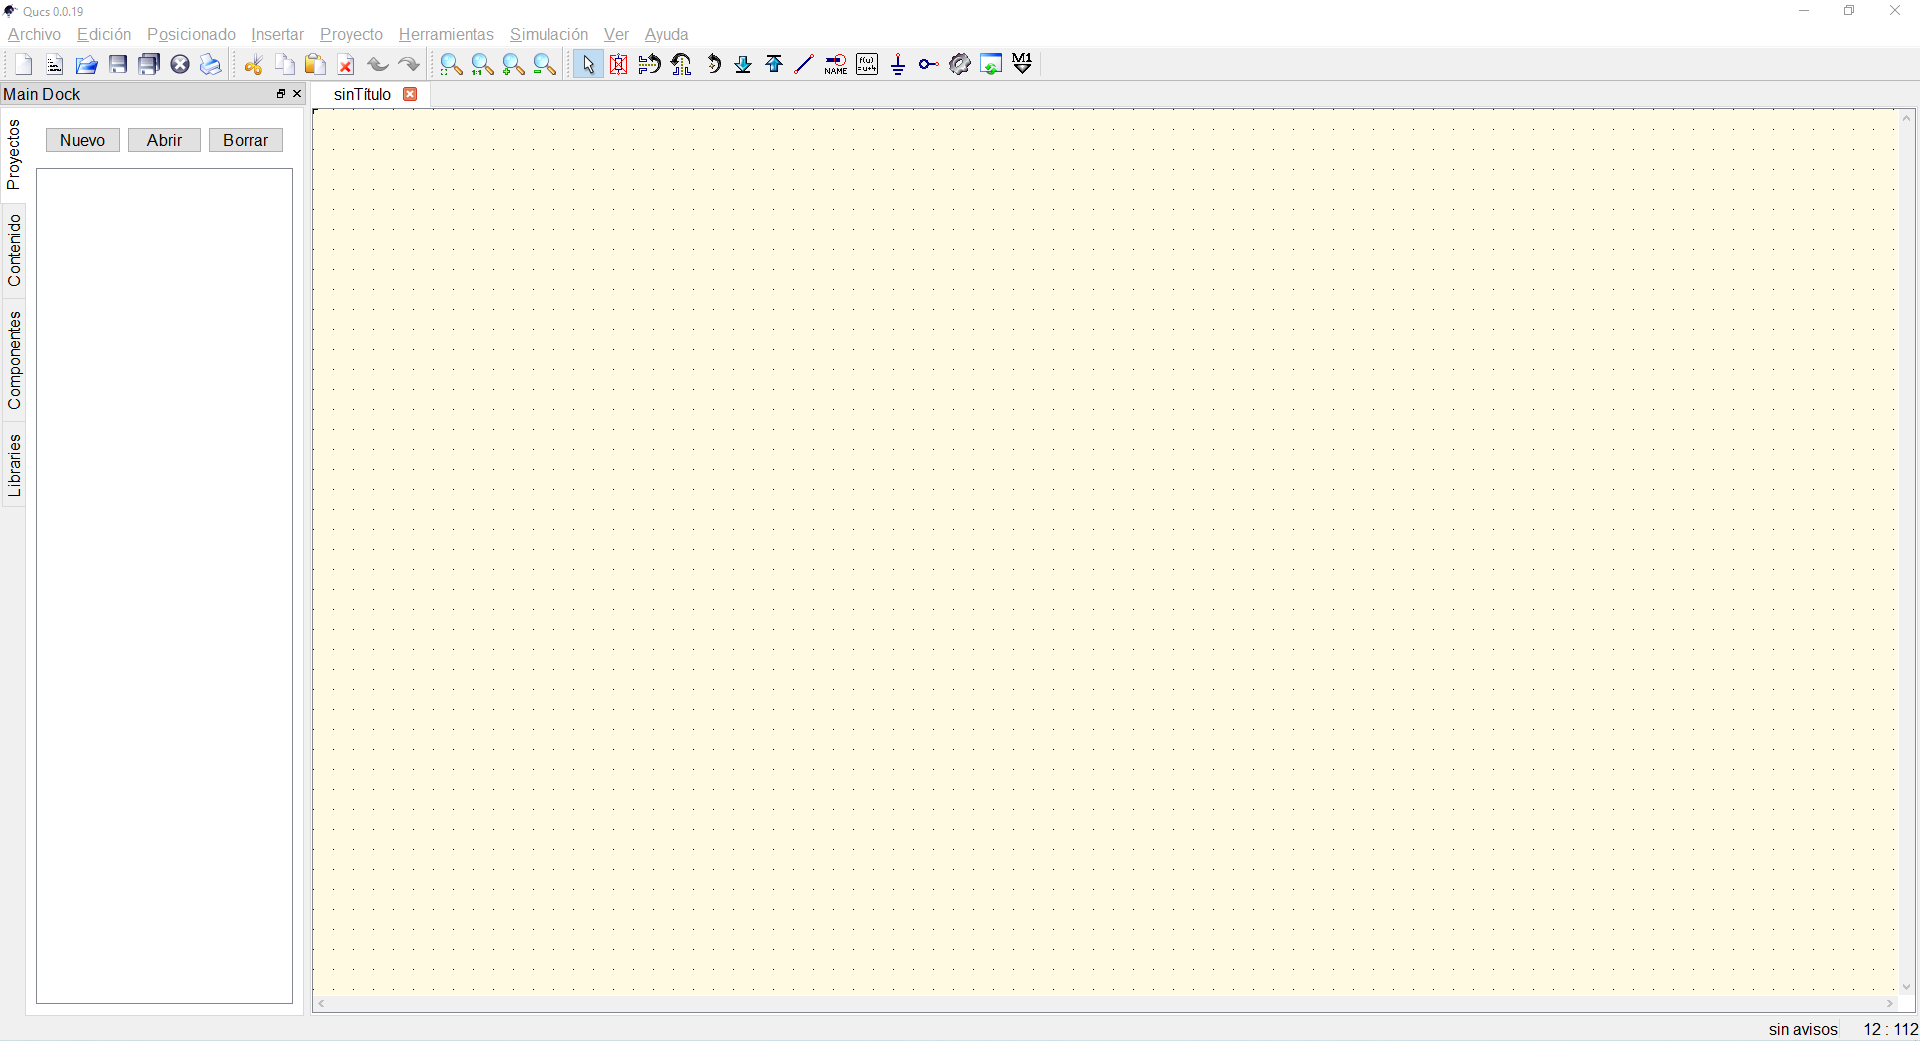
\includegraphics[width=\linewidth]{../figs/qucs1.PNG}
    \caption{Ventana principal de \qucs}
    \label{fig.qucs1}
\end{figure}

Para empezar a simular circuitos, lo primero que hay que hacer es crear un \texttt{Nuevo proyecto}. Para ello, aparecen dos opciones:
\begin{itemize}
    \item Darle al botón \texttt{Nuevo}, que aparece en la parte superior izquierda en la pestaña de \texttt{Proyectos}
    \item Seguir la ruta \texttt{Proyecto} $\rightarrow$ \texttt{Nuevo proyecto}
\end{itemize}
En cualquiera de los dos casos, aparece una nueva ventana donde se pide el nombre del proyecto (Figura~\ref{fig.qucs2}). Se introduce el nombre deseado y se pulsa el botón \texttt{Crear}. Con esto, se abre el proyecto creado y {\qucs} cambia automáticamente a la pestaña de \texttt{Contenido} (Figura~\ref{fig.qucs3}).
\begin{figure}[htbp]
    \centering
    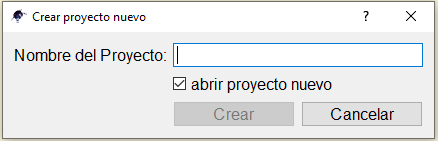
\includegraphics[width=0.35\linewidth]{../figs/qucs2.PNG}
    \caption{Creación de un nuevo proyecto en \qucs}
    \label{fig.qucs2}
\end{figure}
\begin{figure}[htbp]
    \centering
    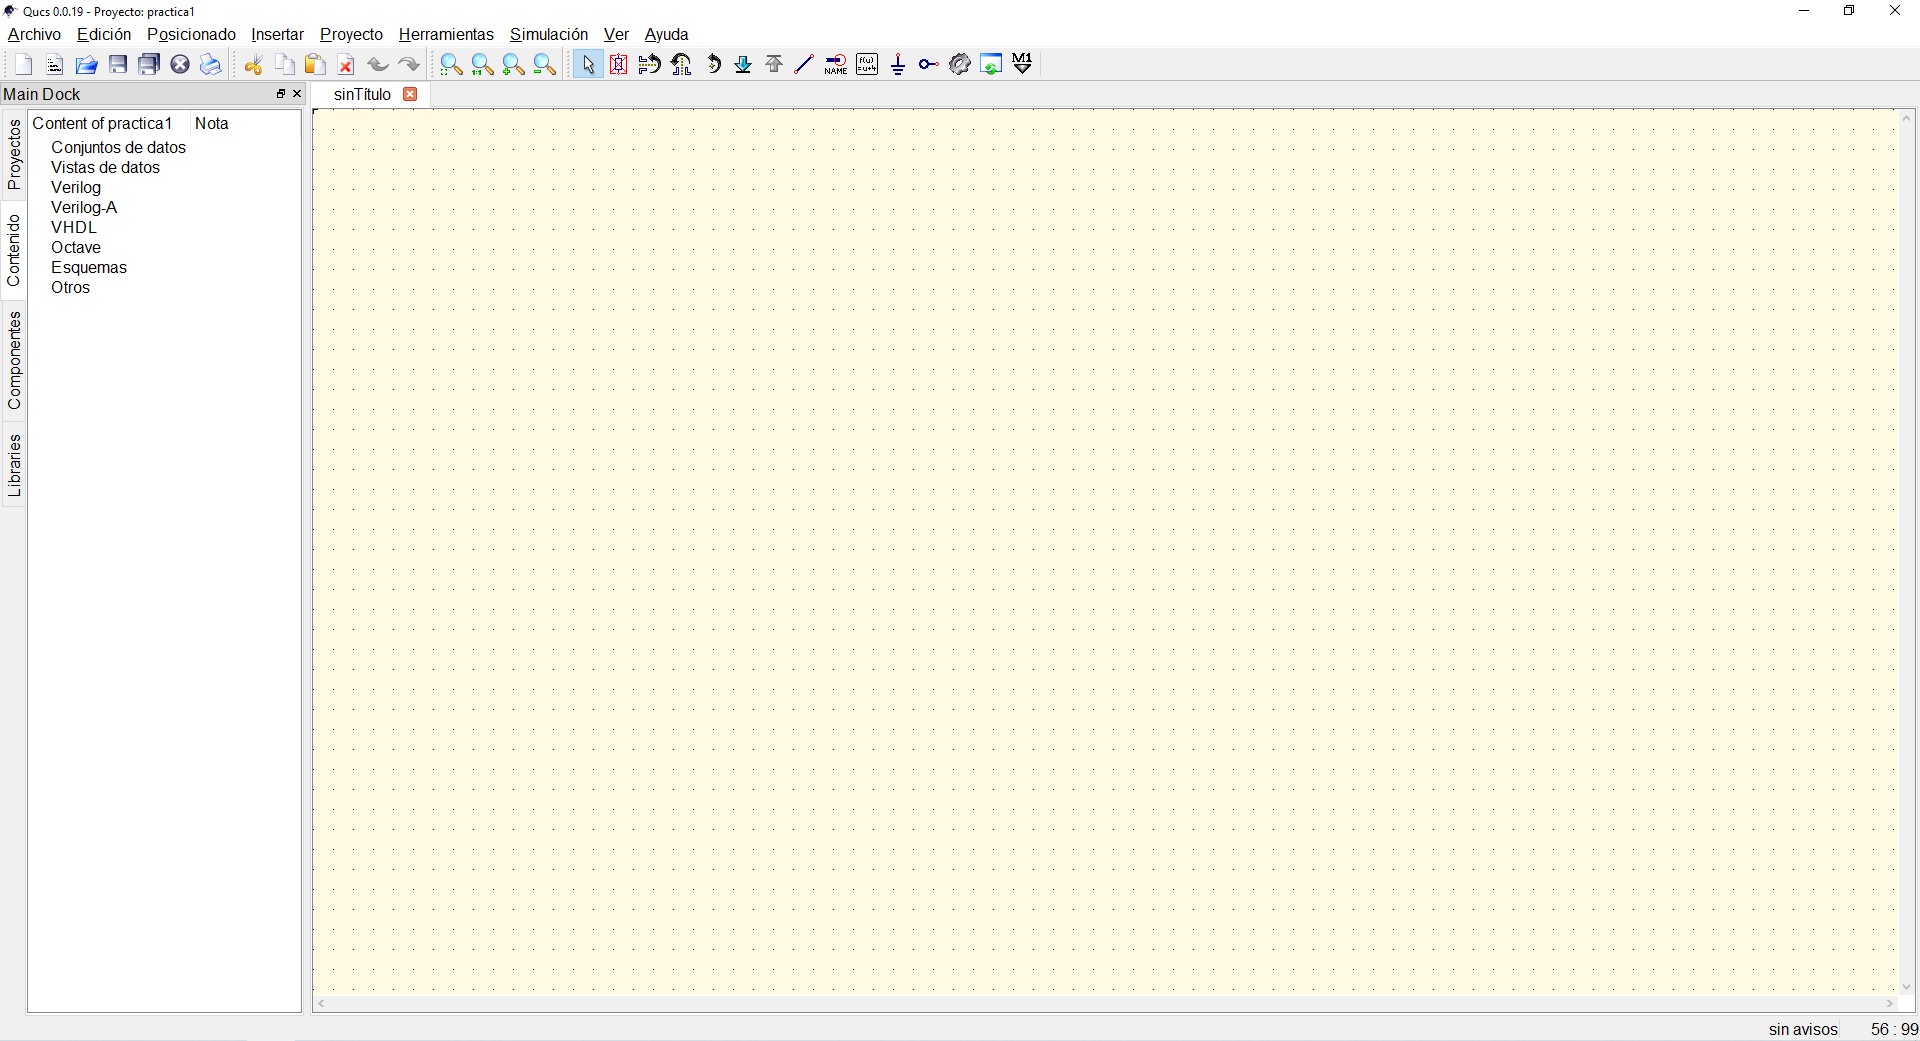
\includegraphics[width=\linewidth]{../figs/qucs3.PNG}
    \caption{Se ha creado un nuevo proyecto vacío}
    \label{fig.qucs3}
\end{figure}

En esta pestaña de \texttt{Contenido}, se muestran todos los datos relacionados con el proyecto. En la parte de la derecha, se muestra un esquema vacío y sin título. En esa zona es donde se incluyen los diferentes componentes que forman el circuito, que se pueden encontrar en la pestaña \texttt{Componentes} de la izquierda (Figura~\ref{fig.qucs4}).
\begin{figure}[htbp]
    \centering
    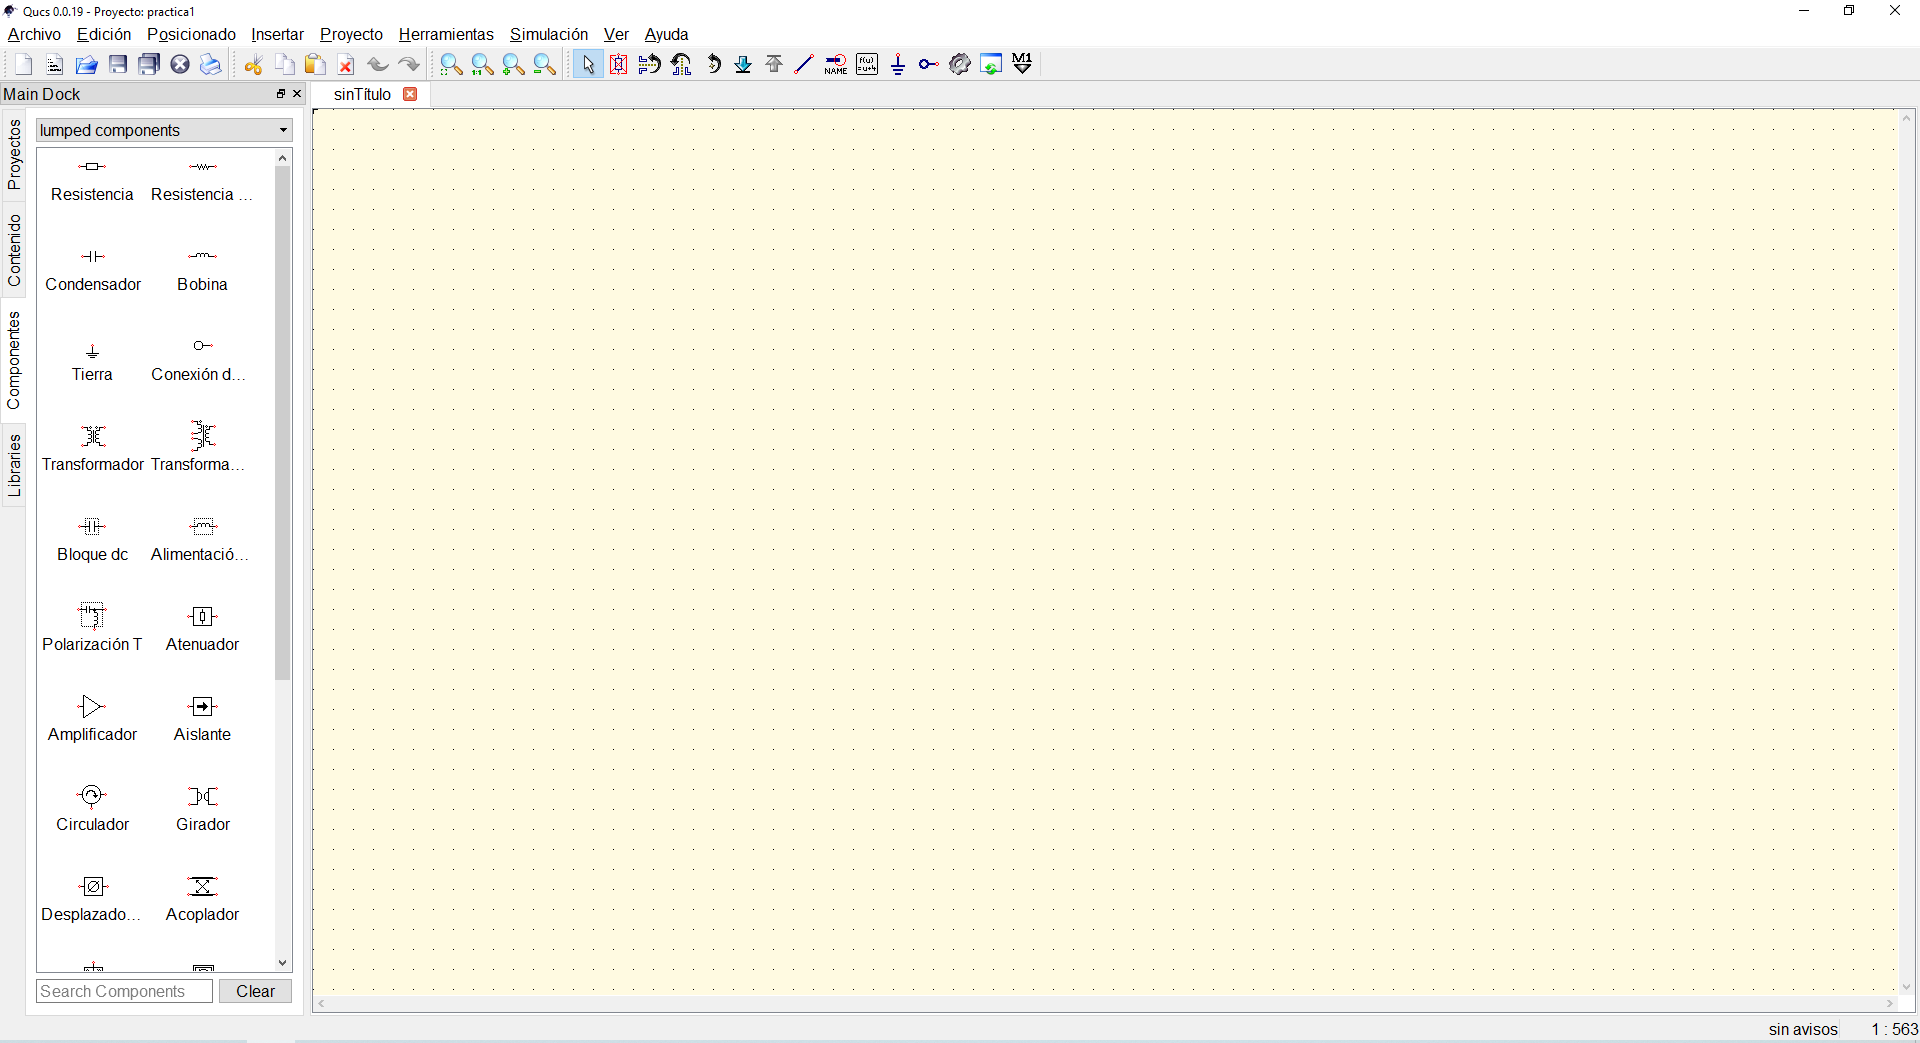
\includegraphics[width=\linewidth]{../figs/qucs4.PNG}
    \caption{Pestaña de \texttt{Componentes}}
    \label{fig.qucs4}
\end{figure}

\section{Simulación en CC -- Divisor de tensión}

Para aprender el manejo básico de \qucs, se realiza un circuito en CC para comprobar el divisor de tensión. Se trata de un circuito formado por una fuente de tensión de CC y dos resistencias en serie. El nombre del proyecto es \texttt{divisorTension}. En la pestaña de \texttt{Componentes}, se eligen los elementos a insertar y se arrastran hasta la ventana del esquema para ubicarlos en la posición deseada. 

Para enlazar los componentes, es necesario cablearlos. Puede hacerse:
\begin{itemize}
    \item Utilizando el icono de cablear (marcado en rojo en la Figura~\ref{fig.qucs5})
    \item Con la secuencia de teclas \texttt{Ctrl} $+$ \texttt{E}
\end{itemize}
    \begin{figure}[htbp]
        \centering
        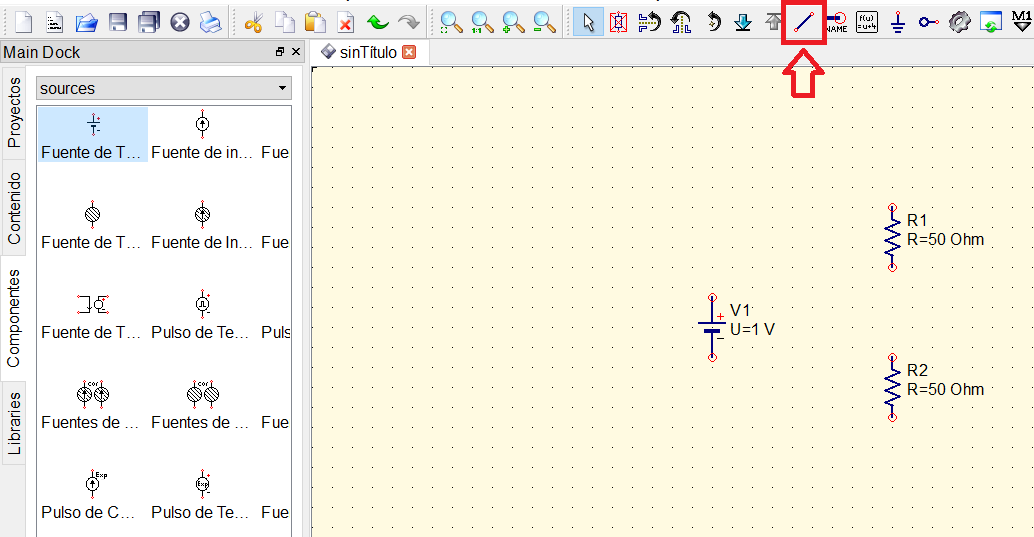
\includegraphics[width=0.7\linewidth]{../figs/qucs5.png}
        \caption{Icono para cablear en \qucs}
        \label{fig.qucs5}
    \end{figure}

Para dejar de cablear, se debe pulsar \texttt{Esc}.

Es necesario incluir también un nudo de referencia (tierra/masa), que puede encontrarse:
\begin{itemize}
    \item Utilizando el icono de tierra (marcado en rojo en la Figura~\ref{fig.qucs6})
    \item Con la secuencia de teclas \texttt{Ctrl} $+$ \texttt{G}
    \item Entre los \texttt{lumped components}
\end{itemize}
    \begin{figure}[htbp]
        \centering
        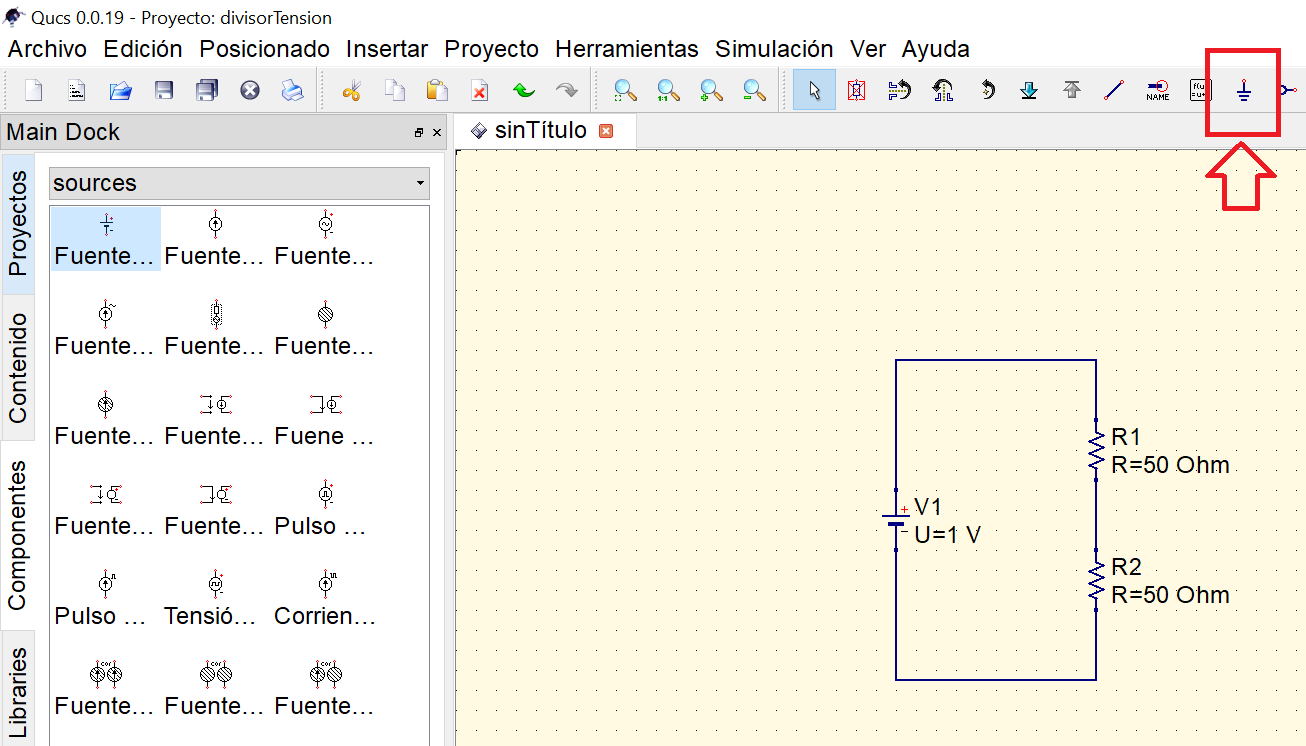
\includegraphics[width=0.7\linewidth]{../figs/qucs6.png}
        \caption{Icono de tierra en \qucs}
        \label{fig.qucs6}
    \end{figure}

A continuación, hay que elegir el tipo de simulación que se va a realizar, que se realiza insertando un bloque de simulación en el esquema. Estos bloques de simulación se encuentran en la pestaña \texttt{Componentes}, eligiendo en el desplegable \texttt{simulations}, Figura~\ref{fig.qucs7}. En este caso, se va a realizar una simulación de corriente continua, por lo que se elige el bloque de \texttt{simulación dc} y se coloca en el esquema.  
\begin{figure}[htbp]
    \centering
    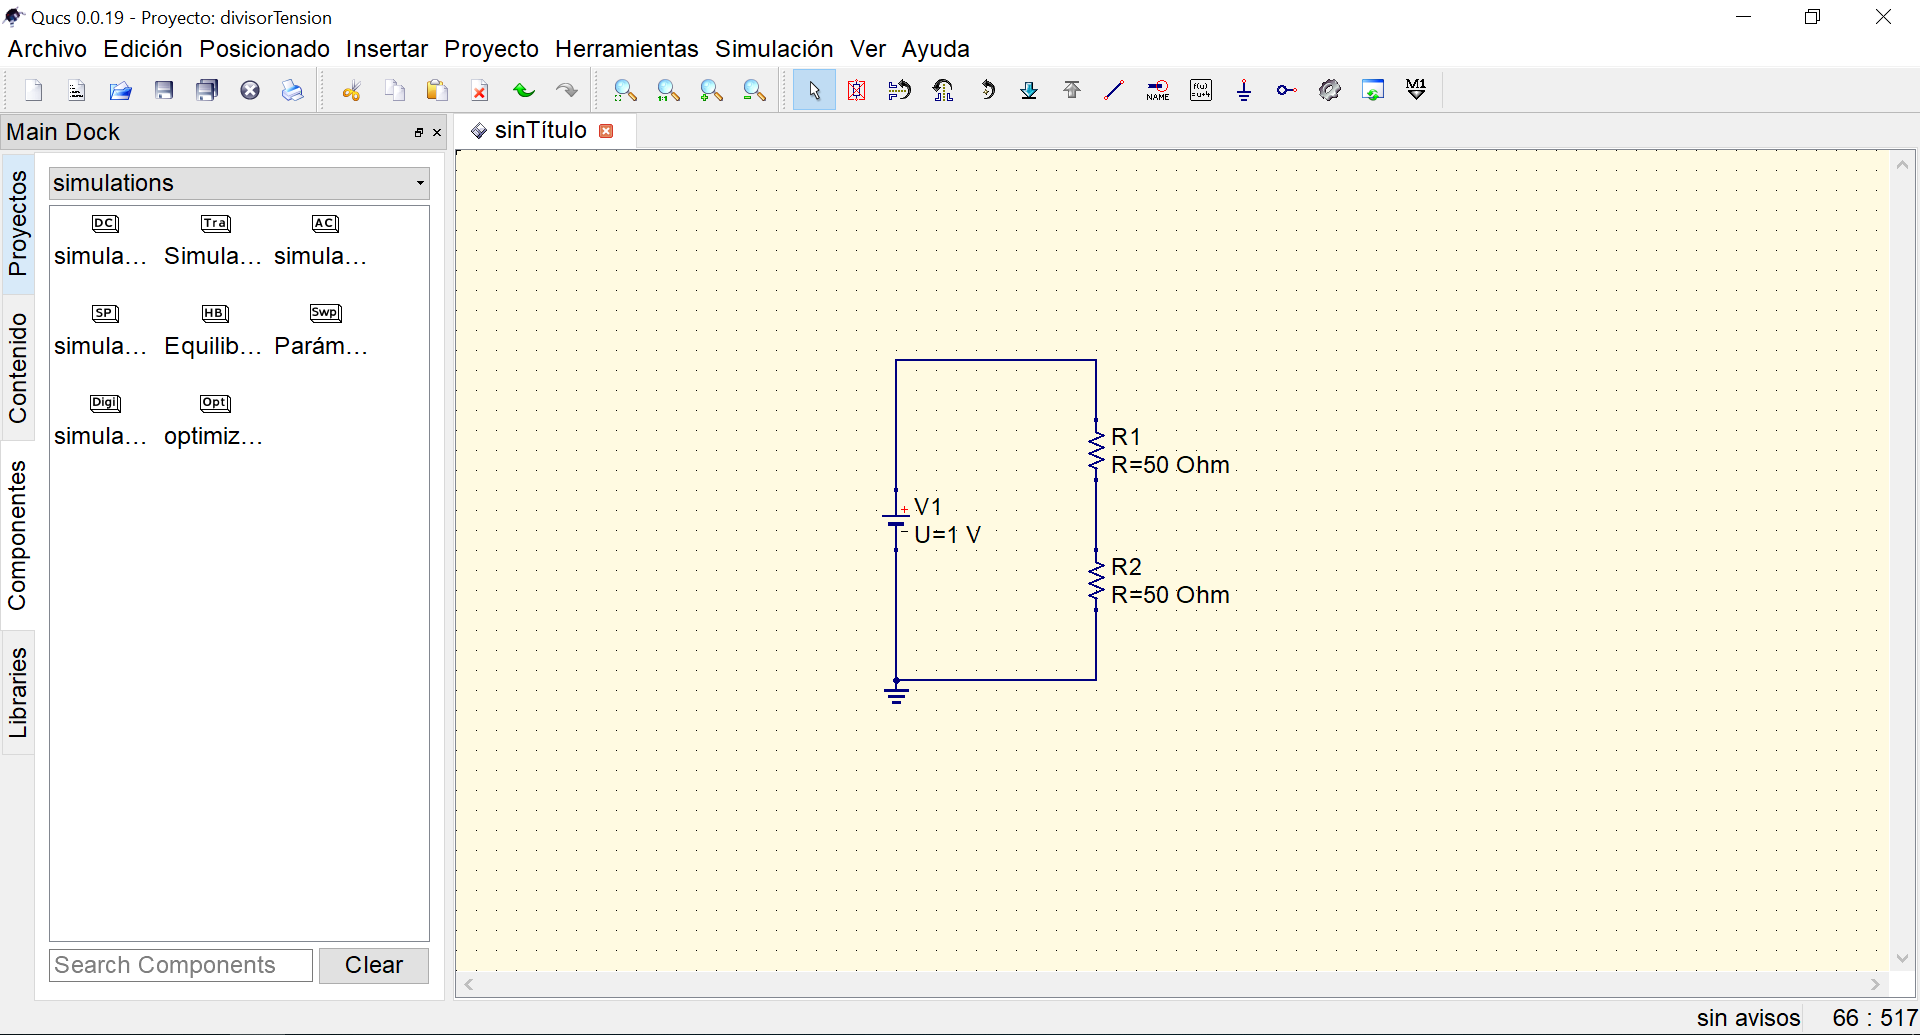
\includegraphics[width=\linewidth]{../figs/qucs7.PNG}
    \caption{Bloques de simulación en \qucs}
    \label{fig.qucs7}
\end{figure}

Finalmente, hay que decidir qué es lo que se quiere medir. En este caso, quiere conocerse la tensión que hay entre ambas resistencias. Para ello, hay que insertar una sonda (\texttt{etiqueta del cable}) entre las dos resistencias por alguno de los siguientes métodos:
\begin{itemize}
    \item Utilizando el icono de etiqueta (marcado en rojo en la Figura~\ref{fig.qucs8})
    \item Con la secuencia de teclas \texttt{Ctrl} $+$ \texttt{L}
    \item Haciendo doble click en el cable en cuestión
\end{itemize}
    \begin{figure}[htbp]
        \centering
        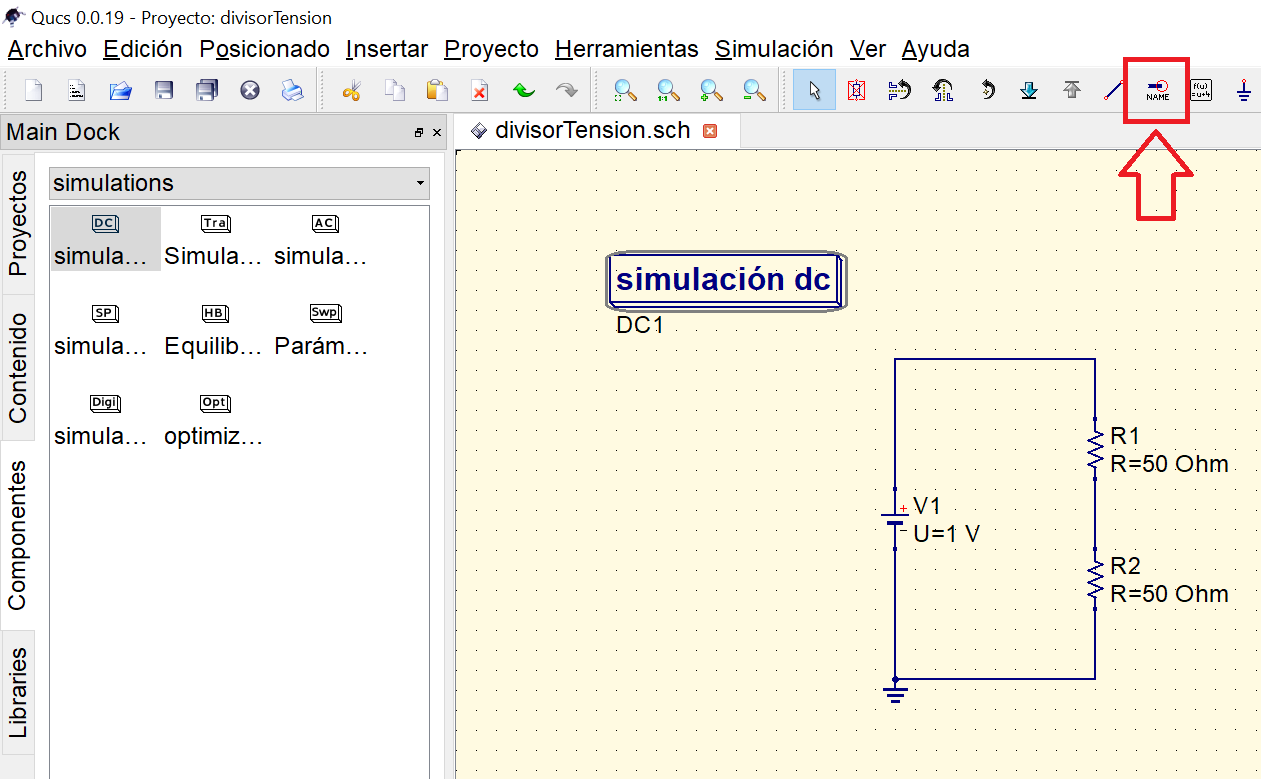
\includegraphics[width=0.5\linewidth]{../figs/qucs8.png}
        \caption{Icono de etiqueta en \qucs}
        \label{fig.qucs8}
    \end{figure}

Con cualquiera de esas opciones, y tras seleccionar el cable al que se le quiere incluir la etiqueta, aparece una ventana donde insertar el nombre del nudo (Figura~\ref{fig.qucs9}). Para asignar el nombre, se deberá escribir éste en el cuadro de diálogo (en este caso, \texttt{divisor}) y pulsar en el botón \texttt{Aceptar}. Con esto, se termina el esquema del circuito, que se guardará mediante \texttt{Archivo} $\rightarrow$ \texttt{Guardar}. 
\begin{figure}[htbp]
    \centering
    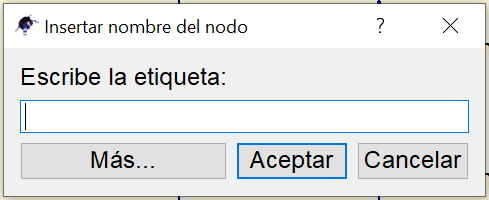
\includegraphics[width=0.35\linewidth]{../figs/qucs9.PNG}
    \caption{Insertar nombre de un nudo en \qucs}
    \label{fig.qucs9}
\end{figure}

Para iniciar la simulación:
\begin{itemize}
    \item Se utiliza el icono de simulación (marcado en rojo en la Figura~\ref{fig.qucs10})
    \item Con la tecla \texttt{F2}
    \item Mediante la ruta \texttt{Simulación} $\rightarrow$ \texttt{Simular}
\end{itemize}
    \begin{figure}[htbp]
        \centering
        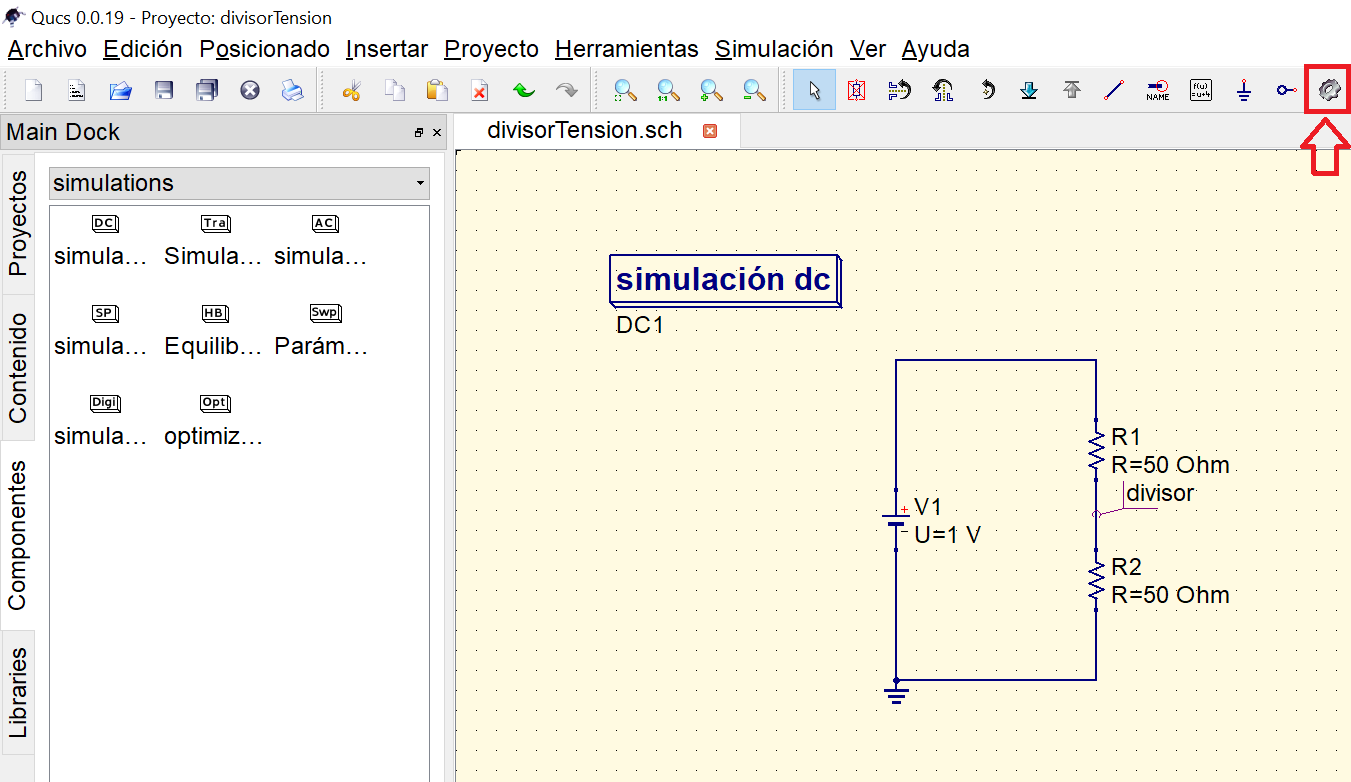
\includegraphics[width=0.7\linewidth]{../figs/qucs10.png}
        \caption{Icono de simular en \qucs}
        \label{fig.qucs10}
    \end{figure}

Con cualquiera de estas opciones, se realiza la simulación, y {\qucs} muestra la pantalla de datos relacionada, que tiene una extensión \texttt{.dpl}, así como cambiar automáticamente el desplegable a \texttt{diagrams} (Figura~\ref{fig.qucs11}). 
\begin{figure}[htbp]
    \centering
    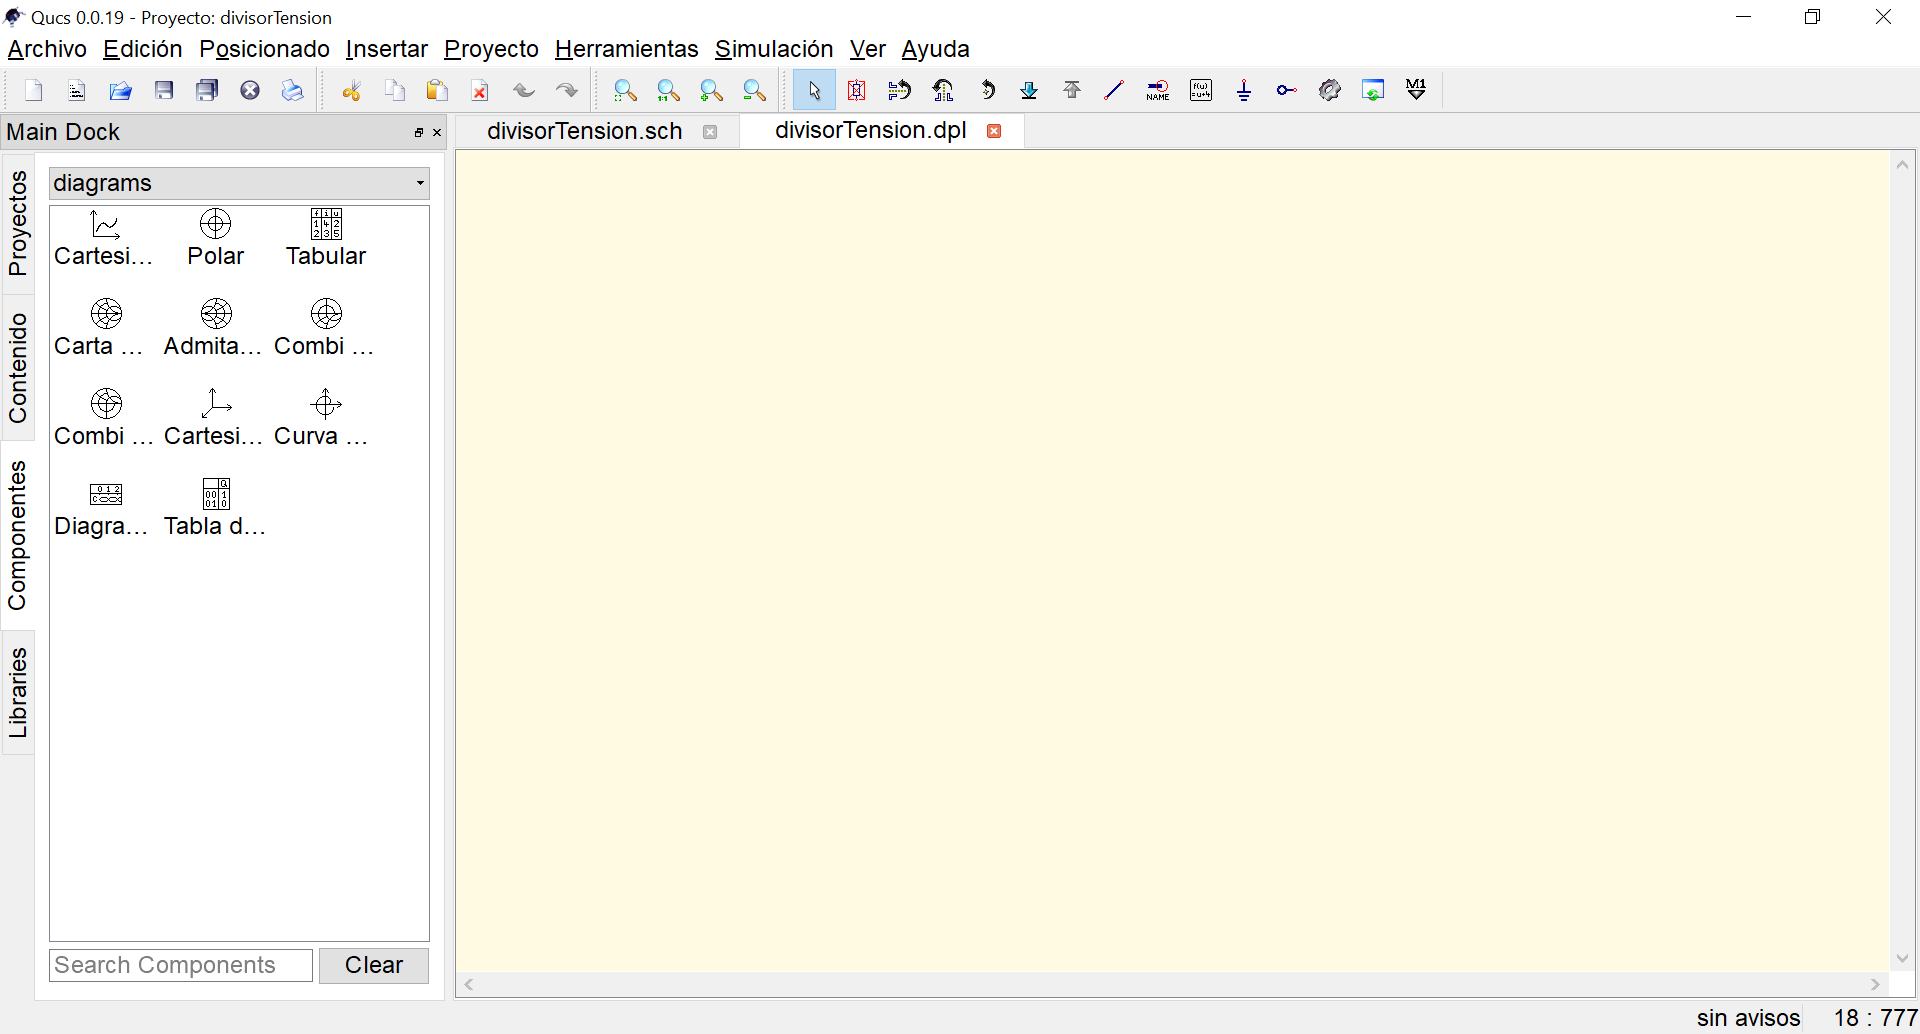
\includegraphics[width=\linewidth]{../figs/qucs11.PNG}
    \caption{Pantalla de datos tras simulación}
    \label{fig.qucs11}
\end{figure}

Para mostrar los resultados de la simulación, se debe elegir alguna de las opciones de las mostradas en el desplegable de \texttt{diagrams}. En este ejemplo, se usará la opción \texttt{Tabular}, que muestra la lista de valores de la simulación. Una vez incluida en la pantalla de datos tras la simulación, aparece la ventana de la Figura~\ref{fig.qucs12}. Puesto que lo que se quiere ver es la tensión del divisor, se selecciona \texttt{divisor.V} del Conjunto de Datos, apareciendo en el cuadro de Gráfico (Figura~\ref{fig.qucs13}). 
\begin{figure}[htbp]
    \centering
    \subfigure[Ventana de opciones de \texttt{Tabular}]{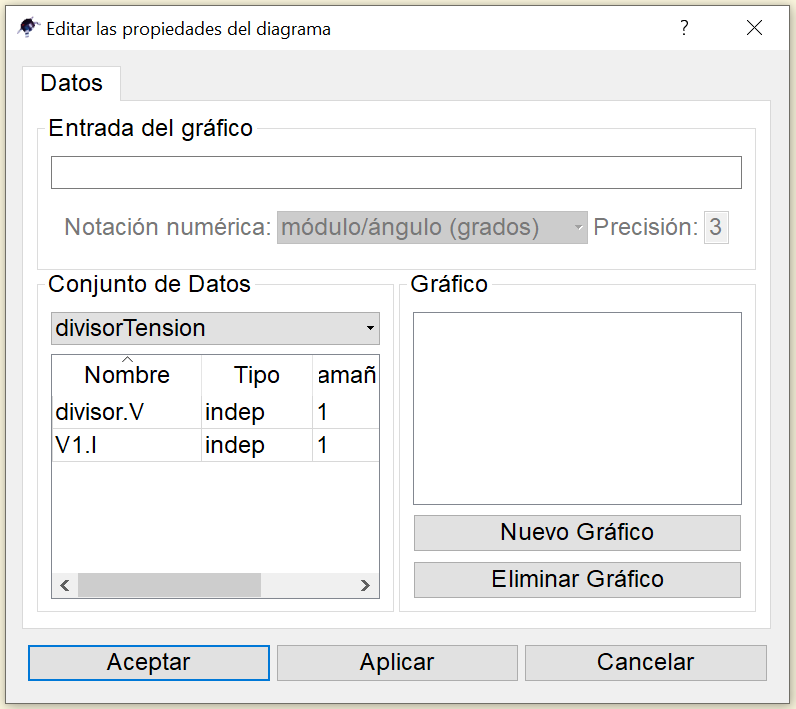
\includegraphics[width=0.48\linewidth]{../figs/qucs12.PNG}\label{fig.qucs12}}\hfill
    \subfigure[Gráfico a mostrar]{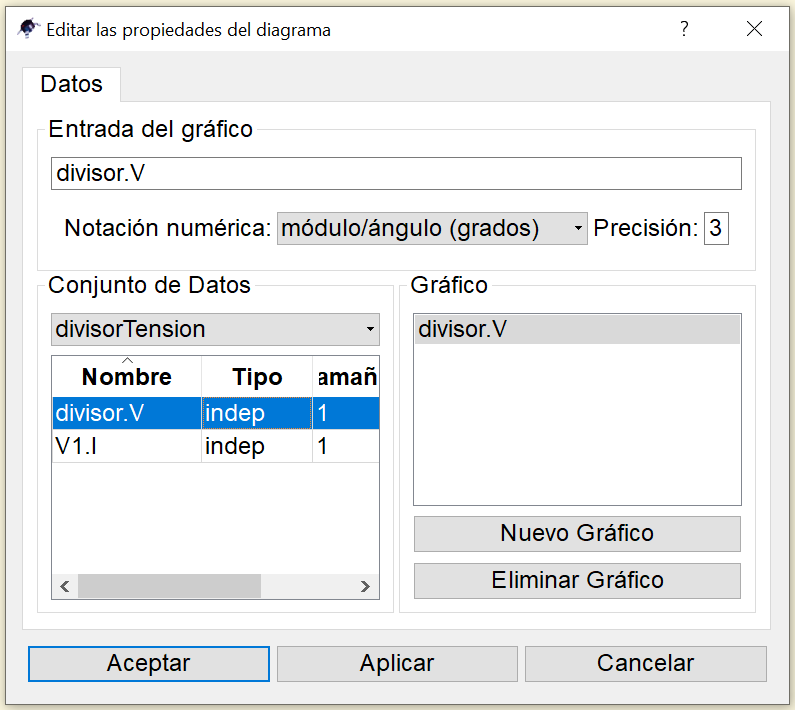
\includegraphics[width=0.48\linewidth]{../figs/qucs13.PNG}\label{fig.qucs13}}
    \caption{Inserción de gráficos tras simulación}
    \label{fig.ventana}
\end{figure}

La otra opción disponible (\texttt{V1.I}) es la corriente de la fuente de tensión. Nótese que únicamente los elementos que aparecen en el cuadro de Conjunto de Datos son los que se pueden representar\footnote{Según el tipo de simulación, se pueden encontrar los siguientes tipos de Conjunto de Datos:
\begin{itemize}
    \item \texttt{nudo.V} --– simulación DC, tensión en el nudo \texttt{nudo}
    \item \texttt{nombre.I} –-- simulación DC, corriente que circula por el componente \texttt{nombre}
    \item \texttt{nudo.v} --– simulación AC, tensión en el nudo \texttt{nudo}
    \item \texttt{nombre.i} –-- simulación AC, corriente que circula por el componente \texttt{nombre}
    \item \texttt{nudo.Vt} –-- simulación transitorio, tensión en el nudo \texttt{nudo}
    \item \texttt{nombre.It} --– simulación transitorio, corriente que circula por el componente \texttt{nombre}
\end{itemize}}. En función del tipo de gráfico que se vaya a utilizar, se tienen diferentes opciones de configuración. En el caso de \texttt{Tabular}, se puede elegir la precisión y el tipo de notación numérica. Una vez configurado, se pulsa \texttt{Aceptar} y se obtiene la tabla de resultados (Figura~\ref{fig.qucs14}), donde se ve que el valor de la tensión en el nudo \texttt{divisor.V} son \qty{0.5}{\volt}. Este resultado es el esperado, dado que el valor de ambas resistencias es el mismo y la fuente de tensión genera \qty{1}{\volt}. 
\begin{figure}[htbp]
    \centering
    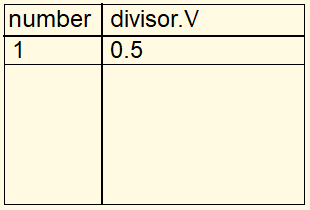
\includegraphics[width=0.25\linewidth]{../figs/qucs14.PNG}
    \caption{Tabla de resultados}
    \label{fig.qucs14}
\end{figure}

Si una vez realizada la simulación se quisiera cambiar alguno de los datos iniciales del esquema, se debe cambiar a la pestaña de extensión \texttt{.sch} y seleccionar el elemento a modificar. Supóngase que se quieren reducir los valor de las resistencias ($R1$ a \qty{1}{\ohm} y $R2$ a \qty{3}{\ohm}). Haciendo doble click en cada resistencia, aparece la ventana de la Figura~\ref{fig.qucs15}, donde pueden cambiarse los valores especificados; en este caso, únicamente se reducen los valores de las resistencias. 
\begin{figure}[htbp]
    \centering
    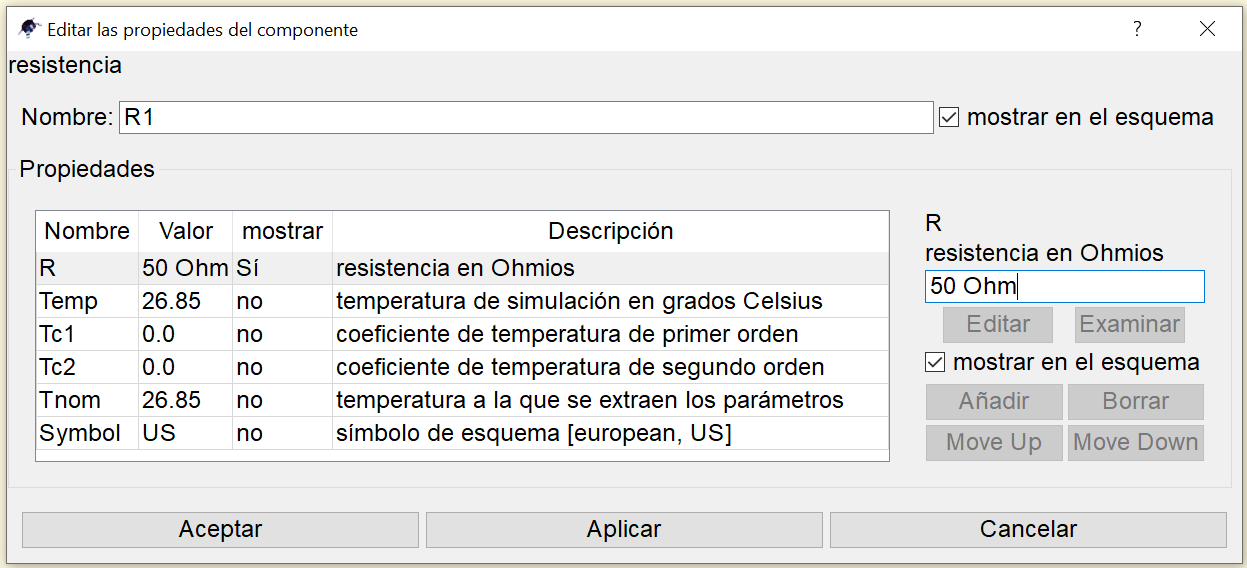
\includegraphics[width=0.9\linewidth]{../figs/qucs15.PNG}
    \caption{Ventana para editar propiedades de un componente}
    \label{fig.qucs15}
\end{figure}

Repitiendo ahora la simulación para el nuevo circuito (Figura~\ref{fig.qucs16}), se tiene que la tensión en el nudo \texttt{divisor} es de \qty{0.75}{\volt}, tal y como se muestra en la Figura~\ref{fig.qucs17}. Los diagramas pueden incluirse también en los esquemas, no es necesario que estén en la pantalla de datos (extensión \texttt{.dpl})
\begin{figure}
    \centering
    \subfigure[Nuevo circuito]{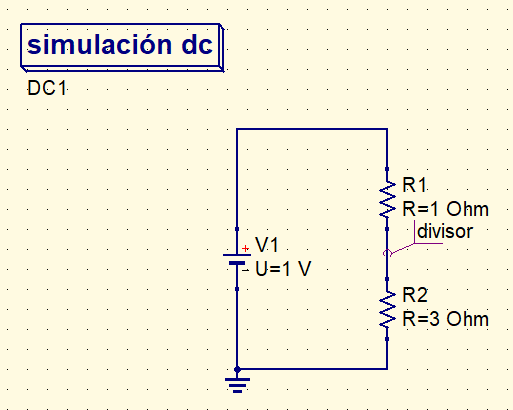
\includegraphics[width=0.3\linewidth]{../figs/qucs16.PNG}\label{fig.qucs16}}\hfil
    \subfigure[Resultado]{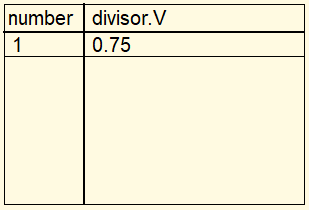
\includegraphics[width=0.25\linewidth]{../figs/qucs17.PNG}\label{fig.qucs17}}
    \caption{Nuevo circuito y resultados de la simulación}
\end{figure}

\section{Simulación en CC -- Divisor de corriente}

Ahora se hace otra simulación para comprobar un divisor de corriente. Se trata de un circuito formado por una fuente de tensión de CC y dos resistencias en paralelo. El nombre del proyecto es \texttt{divisorCorriente}. En la pestaña de \texttt{Componentes}, se eligen los elementos a insertar y se arrastran hasta la ventana del esquema para ubicarlos en la posición deseada, enlazándolos y añadiendo el nudo de tierra. En este caso, se va a añadir también una sonda de corriente para cada rama (se encuentra en el desplegable de \texttt{probes}), y se inserta el bloque de \texttt{simulación dc}. El circuito queda como se muestra en la Figura~\ref{fig.qucs18}.
\begin{figure}[htbp]
    \centering
    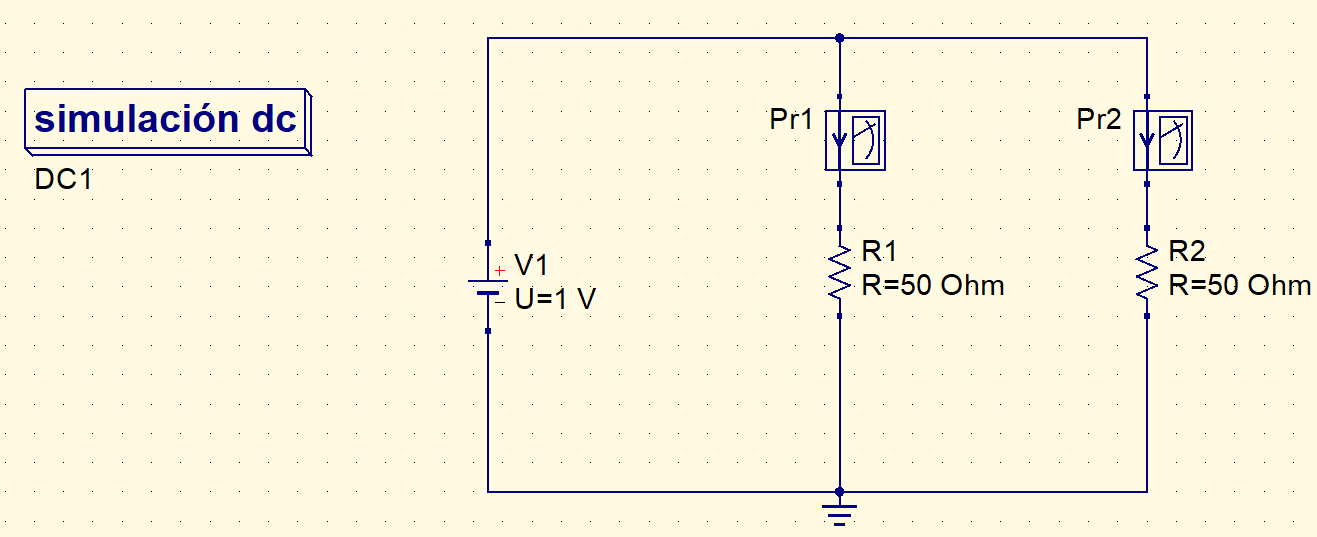
\includegraphics[width=0.5\linewidth]{../figs/qucs18.PNG}
    \caption{Circuito del divisor de corriente}
    \label{fig.qucs18}
\end{figure}

Con esto, se ejecuta la simulación, y se muestra, con la opción \texttt{Tabular}, las corrientes que circulan por ambas resistencias, que es \qty{0.02}{\ampere}, tal y como se obtiene mediante la simulación (Figura~\ref{fig.qucs19}).
\begin{figure}[htbp]
    \centering
    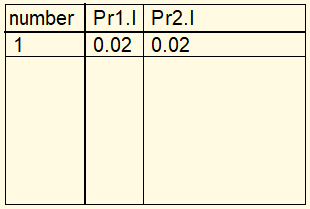
\includegraphics[width=0.25\linewidth]{../figs/qucs19.PNG}
    \caption{Resultados del divisor de corriente}
    \label{fig.qucs19}
\end{figure}

Cambiando ahora los valor de las resistencias ($R1$ a \qty{0.5}{\ohm} y $R2$ a \qty{1}{\ohm}) y repitiendo la simulación para el nuevo circuito (Figura~\ref{fig.qucs20}), se tiene que las corrientes en cada rama son \qty{2}{\ampere} y \qty{1}{\ampere}, tal y como se muestra en la Figura~\ref{fig.qucs21}.
\begin{figure}
    \centering
    \subfigure[Nuevo circuito]{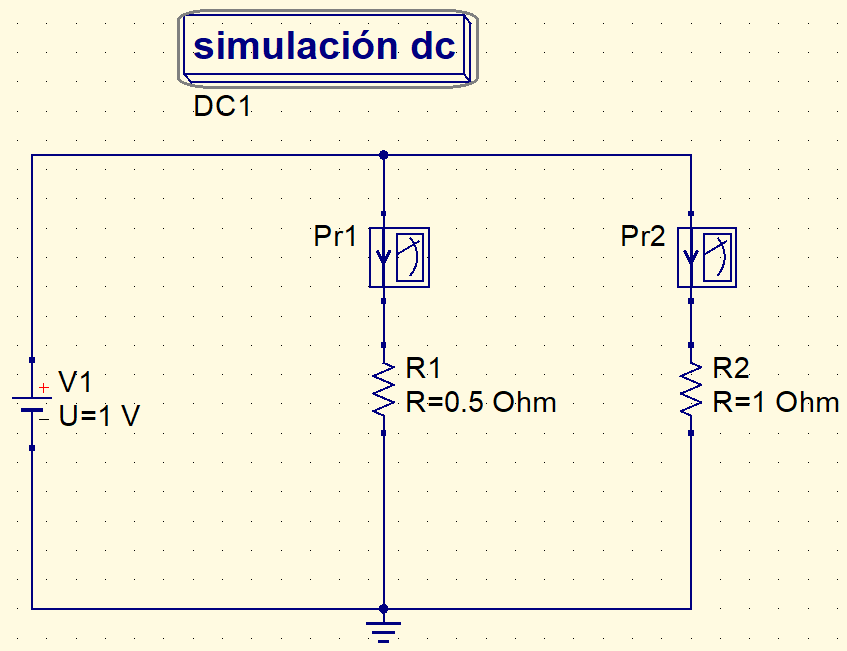
\includegraphics[width=0.3\linewidth]{../figs/qucs20.PNG}\label{fig.qucs20}}\hfil
    \subfigure[Resultado]{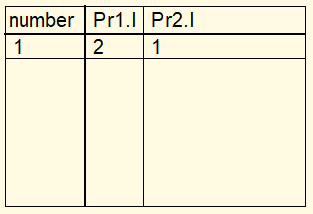
\includegraphics[width=0.25\linewidth]{../figs/qucs21.PNG}\label{fig.qucs21}}
    \caption{Nuevo circuito y resultados de la simulación}
\end{figure}


\section{Simulación en CA -- Divisor de tensión}

Se repiten los circuitos anteriores, pero con CA. Para el divisor de tensión, se incluyen las tres resistencias y una fuente de CA, modificando su frecuencia a \qty{50}{\hertz}. Se enlazan, se añaden dos etiquetas del cable (una para ver la tensión \texttt{total} y otra la del \texttt{divisor}) y se incluye el nudo de tierra. Para hacer la simulación en CA\footnote{Debe tenerse en cuenta que todas las tensiones y corrientes son \textit{valores de pico}.}, hay dos opciones, según lo que interese analizar: 
\begin{itemize}
    \item Si se quiere ver la evolución de la señal en función del tiempo, se usará el bloque de \texttt{simulación transitoria}
    \item Si se quiere ver cómo cambia el valor eficaz de la señal el función de la frecuencia, se usará el bloque de \texttt{simulación ac}
\end{itemize}
\begin{figure}[htbp]
    \centering
    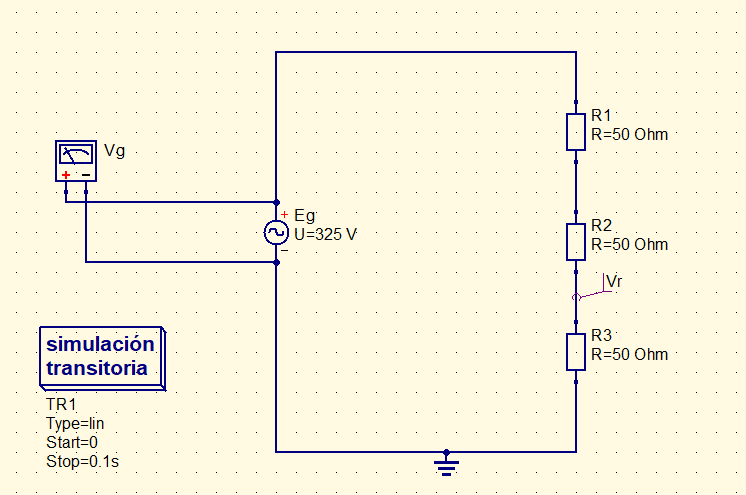
\includegraphics[width=0.4\linewidth]{../figs/qucs_divisorTensionAC.png}
    \caption{Circuito del divisor de tensión en CA}
    \label{fig.qucs22}
\end{figure}
En este caso, se quiere ver la evolución en función del tiempo, por lo que el circuito queda como se muestra en la Figura~\ref{fig.qucs22}. Para ver correctamente la evolución temporal, es necesario modificar los parámetros de la simulación. De manera análoga, haciendo doble click en el bloque, aparece la ventana de la Figura~\ref{fig.qucs23}. Se modifica el parámetro de \texttt{Parada} (a \qty{0.04}{\second}) y el parámetro \texttt{Número} (a 500). {\qucs} automáticamente calcula el parámetro \texttt{Paso} a partir de esta información. 
\begin{figure}[h!]
    \centering
    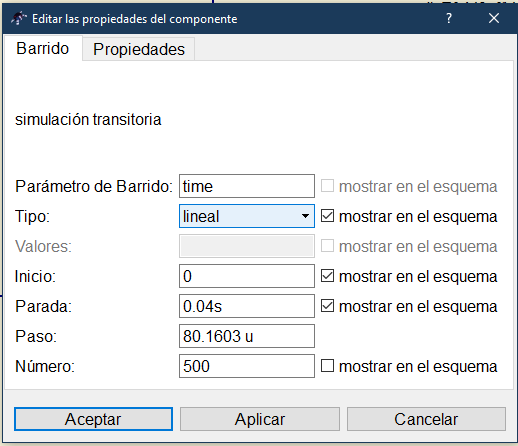
\includegraphics[width=0.45\linewidth]{../figs/qucs_parametrosSimulacion.png}
    \caption{Ventana para editar las propiedades de la simulación}
    \label{fig.qucs23}
\end{figure}

Con esto, se ejecuta la simulación, y se muestra, con la opción \texttt{Cartesiano}, las formas de onda de la Figura~\ref{fig.qucs24}.
\begin{figure}[h!]
    \centering
    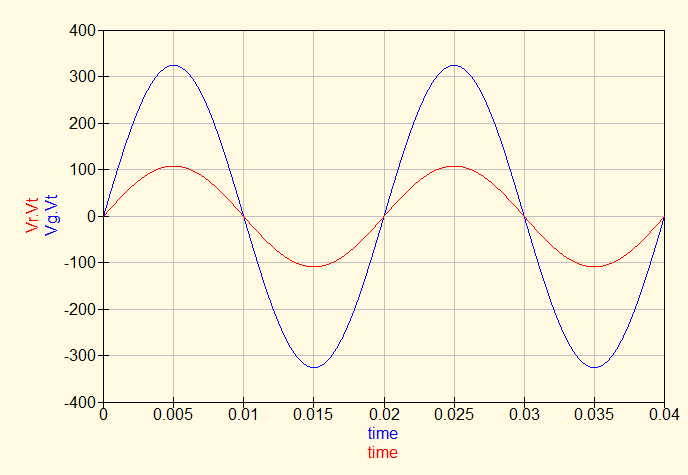
\includegraphics[width=0.85\linewidth]{../figs/qucs_evolucionTemporal.png}
    \caption{Representación de las tensiones en función del tiempo}
    \label{fig.qucs24}
\end{figure}

\clearpage
\section{Ecuaciones}

Con los resultados de las simulaciones se pueden realizar cálculos mediante la inserción de ecuaciones (Figura~\ref{fig.qucs25}). 

\begin{figure}[h!]
    \centering
    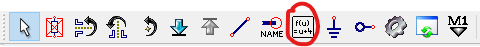
\includegraphics[width=0.85\linewidth]{../figs/qucs_insertarEcuacion.png}
    \caption{Inserción de ecuaciones}
    \label{fig.qucs25}
\end{figure}

Siguiendo con el último circuito, insertemos dos ecuaciones para calcular el valor eficaz de la tensión en el generador y de la tensión en la resistencia $R_3$, y el valor máximo en estos mismos elementos (Figura~\ref{fig.qucs26}).
\begin{figure}[h!]
    \centering
    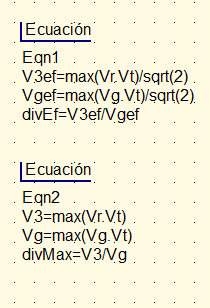
\includegraphics[width=0.25\linewidth]{../figs/qucs_ecuacion.png}
    \caption{Ecuaciones del valor eficaz y valor máximo}
    \label{fig.qucs26}
\end{figure}

En las ecuaciones se pueden definir constantes con un valor determinado, por ejemplo para asignar el valor de un componente circuital. En este caso es importante no incluir unidades dentro de la ecuación, pues serán interpretadas como una variable y la simulación terminará con un error.

Los resultados de estas ecuaciones se pueden mostrar en formato tabla después de ejecutar la simulación del circuito (Figuras~\ref{fig.qucs27} y \ref{fig.qucs28}).

\begin{figure}[h!]
    \centering
    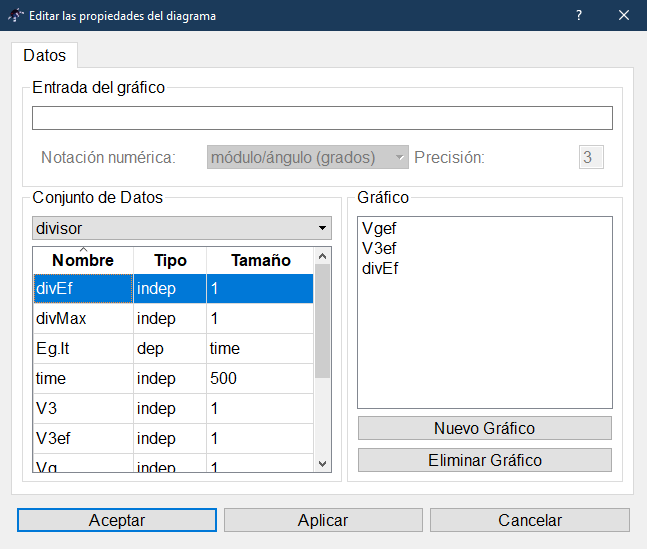
\includegraphics[width=0.45\linewidth]{../figs/qucs_seleccionVariablesEcuacion.png}
    \caption{Selección de las variables de las ecuaciones}
    \label{fig.qucs27}
\end{figure}

\begin{figure}[h!]
    \centering
    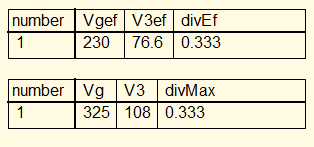
\includegraphics[width=0.25\linewidth]{../figs/qucs_resultadosEcuacion.png}
    \caption{Resultados de las ecuaciones en formato tabular}
    \label{fig.qucs28}
\end{figure}

El documento ``Measurement Expressions Reference Manual''\footnote{Disponible en \url{http://qucs.sourceforge.net/docs/tutorial/functions.pdf}} de {\qucs} detalla las funciones disponibles y el formato de las ecuaciones. 

\section{Barrido de valores de componentes}

En algunos casos es interesante estudiar el comportamiento del circuito para diferentes valores de un componente determinado. {\qucs} permite realizar este análisis de forma sistemática con la simulación \texttt{Sweep} (barrido). Esta simulación se debe añadir después de haber elegido una simulación DC, AC o transitoria. El siguiente ejemplo analiza el comportamiento de un divisor de tensión resistivo para diferentes valores de la resistencia de salida.


En primer lugar, en el circuito señalamos un componente como variable indicando su valor de forma simbólica (Figura~\ref{fig.qucs29}).
\begin{figure}[h!]
    \centering
    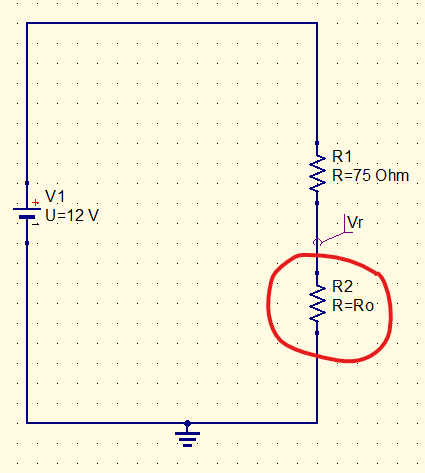
\includegraphics[width=0.25\linewidth]{../figs/qucs_CircuitoSweep.png}
    \caption{Circuito con un componente variable}
    \label{fig.qucs29}
\end{figure}

A continuación, añadimos la simulación \texttt{Sweep} (Figura~\ref{fig.qucs30a}). Para realizar el barrido es necesario configurar este modo de simulación. En el cuadro de diálogo hay que elegir el modo de simulación primario (DC, AC o transitorio), y la variable de estudio  (Figura~\ref{fig.qucs30b}).

\begin{figure}[htbp]
    \centering
    \subfigure[Módulo de simulación sweep sin configurar]{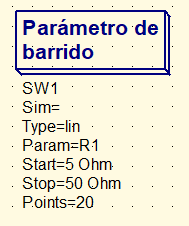
\includegraphics[width=0.25\linewidth]{../figs/qucs_InsertarSweep.png}\label{fig.qucs30a}}\hfill
    \subfigure[Parámetros del barrido]{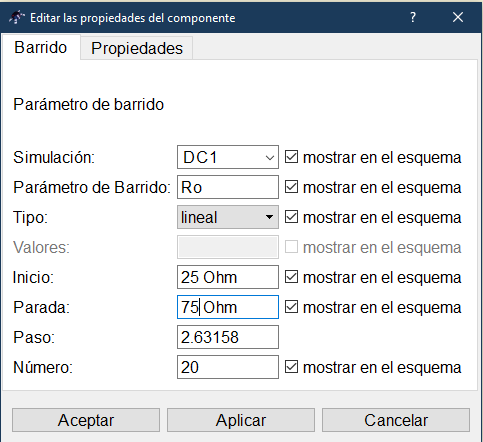
\includegraphics[width=0.45\linewidth]{../figs/qucs_CuadroDialogoSweep.png}\label{fig.qucs30b}}
    \caption{Configuración del barrido}
    \label{fig.qucs30}
\end{figure}

Los resultados del barrido se pueden mostrar de forma gráfica y tabular. Observamos que ahora la variable independiente es la variable de barrido seleccionada (Figura~\ref{fig.qucs31}).
\begin{figure}[h!]
    \centering
    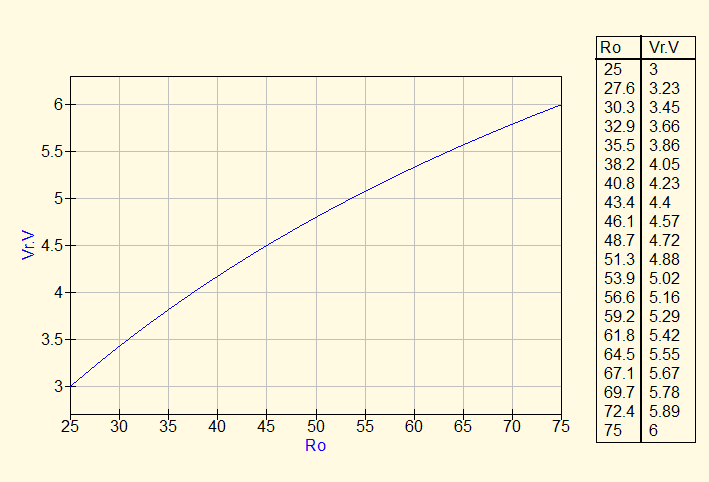
\includegraphics[width=0.85\linewidth]{../figs/qucs_ResultadosSweep.png}
    \caption{Resultados de la simulación Sweep}
    \label{fig.qucs31}
\end{figure}

\end{document}
